%!TEX root = ../thesis.tex
\chapter{Evaluation}\label{evaluation}


\ifpdf
    \graphicspath{{Chapter3/Figs/Raster/}{Chapter3/Figs/PDF/}{Chapter3/Figs/}}
\else
    \graphicspath{{Chapter3/Figs/Vector/}{Chapter3/Figs/}}
\fi


\section{General Notes} \label{evaluationnotes}

In this chapter I provide quantitative and qualitative analysis and comparison of the settings presented in previous chapters, focusing on the:

\begin{itemize}
    \item properties of the optimal \DP strategy for \TwoThinning,
    \item limitations of the \Greedy Strategy for \GraphicalTwoChoice and
    \item patterns in Deep Q-Learning training
\end{itemize} \NOTE{A}{Dimitris, is it okay for the bullet points?}


I compared the strategies across \NumberofRuns runs, showing the average score (final maximum load) of the runs and also the (approximate) $95\%$ confidence interval for the estimated mean score, based on the Central Limit Theorem (CLT). \NOTE{A}{Is it enough to say this? Is it even correct?}. For showing that one strategy is significantly better than the other, I conducted one-tailed Welch's t-tests~\cite{welch1947ttest}, which work for unknown variances, and due to the large number of samples, its normality assumption is also reasonable for the mean score. For higher confidence I conducted Wilcoxon signed-rank tests~\cite{wilcoxon1992test} as well and the results were confirmed.


For space reasons I will usually choose some representative values of $n$ and $m$ to illustrate the general trends, covering different ranges of $n$ and different average final loads $\frac{m}{n}$.


I utilised parallel processing to speed up the execution of Deep Q-Learning policies, which are the bottleneck for thorough and statistically significant evaluation. To exploit the parallelism of the GPU even with the inherently sequential MDP, I ran several (usually $64$) independent samples in parallel. Note that this is much simpler for \TwoThinning and \GraphicalTwoChoice, where the number of steps in the MDP is fixed ($m$) in any execution.


Even with this evaluation speedup, the usability of Deep Q-Learning for large values of $n$ and $m$ is still limited due to the training time. The largest range for which I successfully trained a RL algorithm in at most a day is $n=1000$, $m=1500$, but I decided to focus on slightly smaller values for the evaluation as that is more illustrative and complementary to the literature available. \NOTE{A}{TODO: create some timing plot.} 


I note that there is merit in not just executing several runs with the trained trained Deep Q-Learning model, but also retraining it several times (e.g.\ $20$ runs with each of $5$ independently trained model), because the rewards received during training are also probabilistic. This idea would rather evaluate the robustness of the Deep Q-Learning framework for balls-into-bins settings, but I decided to stick to the more classical single trained model and essentially evaluate the peak performance.


Note that the Dynamic Programming (\DP) strategies are optimal by construction, but they are too slow for larger values of $n$ and $m$ which I denote by Time Limit Exceeded (TLE). The limit was set to $12$ hours of training/hyperparameter tuning/precomputation overall for all the strategies. Also, even though we have the exact expected final maximum load of the \DP strategy, I decided to run it just like the other strategies for fair comparison (e.g.\ large outliers that the \DP strategy takes into account occur very rarely during execution), so it might not always be the best in the comparisons on \NumberofRuns runs (this could be resolved by using the same random seed when evaluating each strategy).


For the \Threshold strategies, I calculated the optimal value of $l$ by modelling it as a Multi-Armed Bandit problem (covered in II Randomised Algorithms)~\cite{katehakis1987multiarmedbandit}, using an $\epsilon$-greedy technique with $\epsilon=0.1$ (details omitted).




\section{\TwoThinning}


\subsection{Comparison of Strategies}\label{two-thinning-comparison}

Now I present a comparison of the \TwoThinning strategies.


\begin{table}[h!]
\centering
\resizebox{\textwidth}{!}{%
\begin{tabular}{|l|c|c|c|c|c|c|c|c|c|}
\hline
                                & \multicolumn{3}{c|}{$n=5$} & \multicolumn{3}{c|}{$n=20$} & \multicolumn{3}{c|}{$n=50$} \\ \hline
Strategy                                & $m=5$ & $m=10$ & $m=25$ & $m=20$ & $m=60$ & $m=400$ & $m=50$ & $m=200$ & $m=2500$ \\ \hline
\AlwaysAccept & 2.30 $\pm$ 0.05 & 3.74 $\pm$ 0.07 & 7.74 $\pm$ 0.11 & 3.18 $\pm$ 0.06 & 6.59 $\pm$ 0.09 & 28.72 $\pm$ 0.20 & 3.78 $\pm$ 0.07 & 9.14 $\pm$ 0.10 & 66.58 $\pm$ 0.31 \\ \hline
\LocalRewardOptimiser & 1.84 $\pm$ 0.04 & 3.00 $\pm$ 0.04 & \textbf{6.07 $\pm$ 0.05} & 2.26 $\pm$ 0.04 & 4.70 $\pm$ 0.05 & 22.46 $\pm$ 0.06 & \textbf{2.59 $\pm$ 0.05} & \textbf{6.32 $\pm$ 0.04} & 53.95 $\pm$ 0.07 \\ \hline
\MeanThinning & 1.87 $\pm$ 0.04 & 3.04 $\pm$ 0.05 & 6.22 $\pm$ 0.06 & 2.53 $\pm$ 0.05 & 5.02 $\pm$ 0.07 & 22.60 $\pm$ 0.09 & 3.02 $\pm$ 0.05 & 6.95 $\pm$ 0.07 & 53.39 $\pm$ 0.10 \\ \hline
\DP & \textbf{1.81 $\pm$ 0.04} & \textbf{2.99 $\pm$ 0.04} & 6.12 $\pm$ 0.05 & \textbf{2.21 $\pm$ 0.04} & \textbf{4.59 $\pm$ 0.05} & TLE & 2.59 $\pm$ 0.05 & TLE & TLE \\ \hline
\DQN & 1.89 $\pm$ 0.04 & 3.02 $\pm$ 0.05 & 6.23 $\pm$ 0.06 & 2.39 $\pm$ 0.05 & 4.84 $\pm$ 0.07 & \textbf{22.18 $\pm$ 0.06} & 2.84 $\pm$ 0.05 & 6.84 $\pm$ 0.07 & \textbf{53.26 $\pm$ 0.09} \\ \hline \Threshold & 2.25 $\pm$ 0.05 & 3.41 $\pm$ 0.06 & 6.64 $\pm$ 0.07 & 2.60 $\pm$ 0.05 & 5.17 $\pm$ 0.06 & 24.18 $\pm$ 0.10 & 3.01 $\pm$ 0.05 & 7.07 $\pm$ 0.07 & 56.52 $\pm$ 0.12 \\ \hline 
\end{tabular}}
\caption{Average maximum load of \TwoThinning strategies with $95\%$ confidence intervals.}
\label{tab:two-thinning-comparison}
\end{table}



The key conclusions from Table~\ref{tab:two-thinning-comparison} are:

\begin{itemize}
    \item The \LocalRewardOptimiser strategy is competitive with the \DP strategy for medium values of $n$ and $m$, even though it only tries avoiding currently maximum loaded bins. For large $\frac{m}{n}$ ratios however, the difference between two non-maximum loaded bins becomes more significant, so the strategy performs worse.
    \item The \DQN strategy is significantly better than the \MeanThinning and \Threshold strategies for all $n\leq 20$, under a largest p-value of $0.034$ and $1.08\cdot 10^{-6}$ respectively. \NOTE{A}{Double check that I am not writing something stupid. In particular, the test I applied assumes that the maximum loads are from a normal distribution and the two distributions have the same variance and none of them are actually true, at least not exactly... How to remedy this?}
    \item The \DQN strategy is consistent, but apart from large values of $n$ and $m$ (when most other strategies fail), it cannot always outperform other strategies. One of the main difficulties for RL is that the impact of a single ball is very subtle and in general, making a small number of bad decisions might not even impact the final maximum load, so strongly negative or strongly positive rewards are not available to the agent.
\end{itemize}

\NOTE{T}{use different for Processes - this will help the reader. Andor: what do you mean? Is a noun missing from your comment?}


\NOTE{A}{Write a bit about the running time of both training and evaluation. DQN would be a bit slower latency-wise but it is bearable. Note that other strategies require no training.}


\NOTE{A}{Add plot showing that \LocalRewardOptimiser doesn't work very well for larger $n$ and $m$. Add general plots for huge $n$ and $m$. Also I can include here the tendencies for the theoretical results, e.g.\ plotting a logarithmic curve. Mention the difficulty in finding the constant factor of those theoretical algorithms.}

\subsection{Theoretical Analysis}

Analysing the optimal strategies for \TwoThinning, I formulated the following conjecture.

\begin{conjecture}\label{conjecture: two-thinning-increasing-threshold}
There exists an optimal (slicing) strategy (i.e. largest possible expected final maximum load) such that its chosen thresholds are non-decreasing during an execution. That is, if for the $i$-th ball the protocol chooses a threshold $x$, then for every later ball of the same execution, a threshold $y\geq x$ is chosen (see Figure \ref{dp-increasing-threshold} for visualisation).
\end{conjecture}


\begin{figure}
\centering
\begin{minipage}[t]{.32\linewidth}
  \centering
  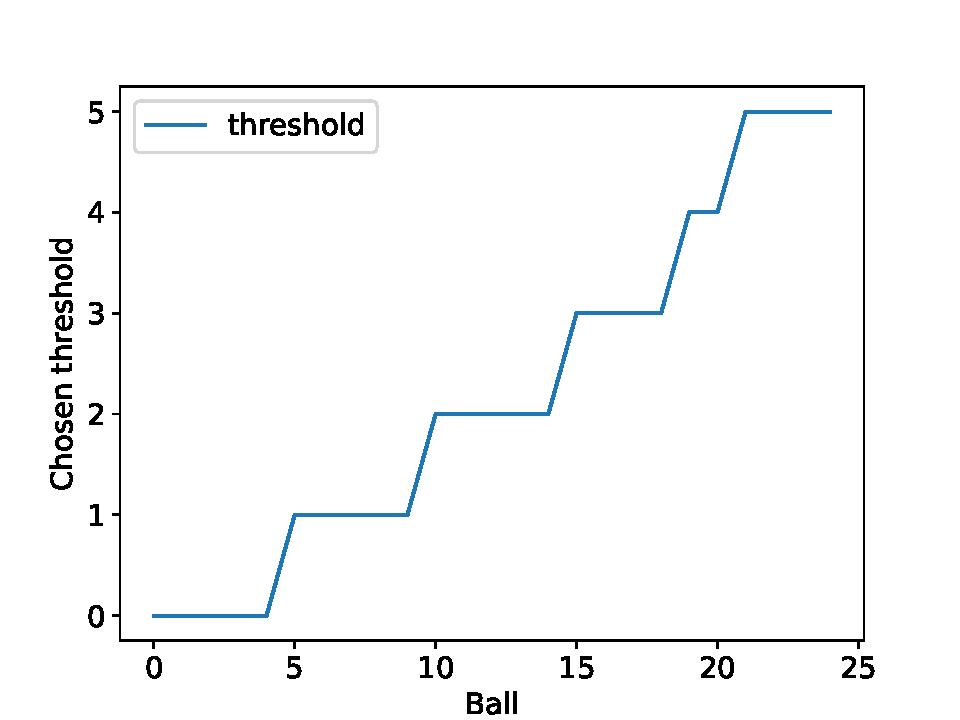
\includegraphics[scale=0.36]{Chapter4/Figs/dp_increasing_threshold_1.pdf}
\end{minipage}\hfill
\begin{minipage}[t]{.32\linewidth}
  \centering
  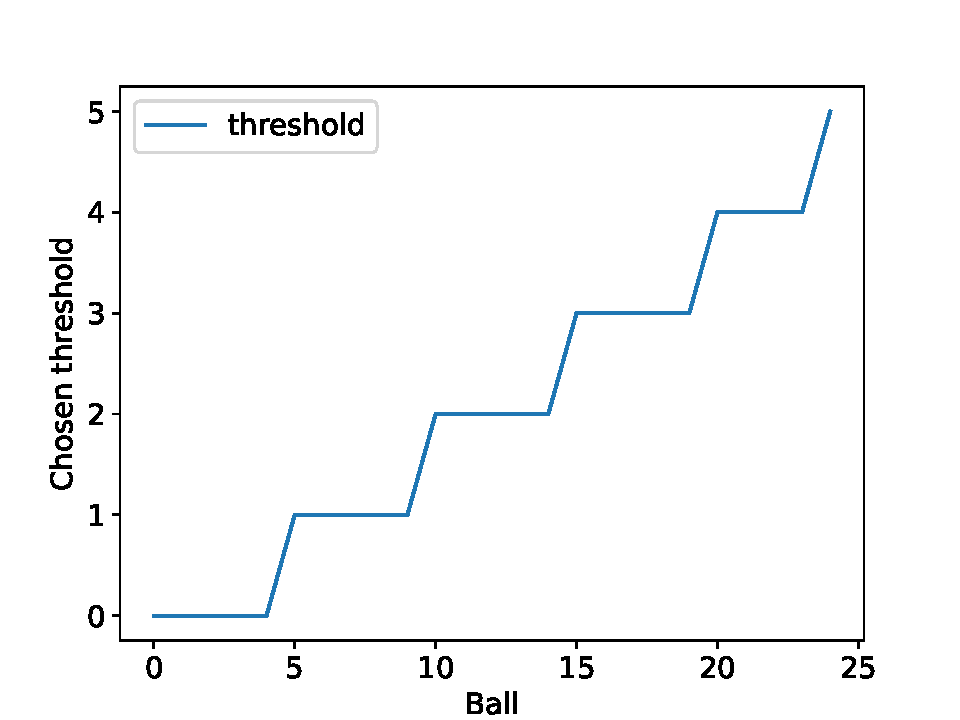
\includegraphics[scale=0.36]{Chapter4/Figs/dp_increasing_threshold_2.pdf}
\end{minipage}\hfill
\begin{minipage}[t]{.32\linewidth}
  \centering
  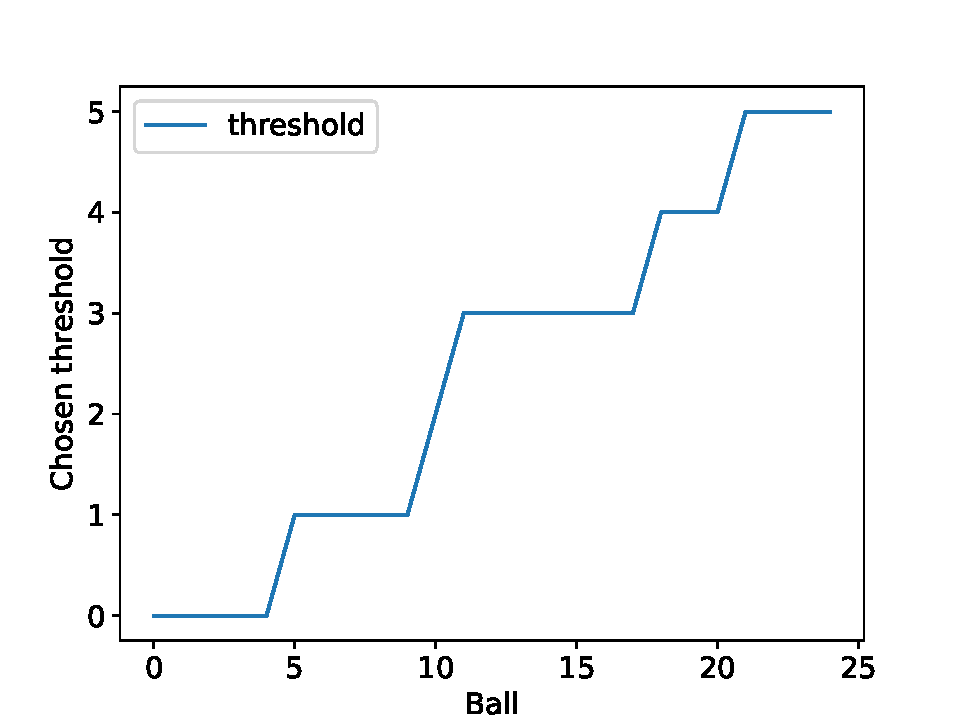
\includegraphics[scale=0.36]{Chapter4/Figs/dp_increasing_threshold_3.pdf}
\end{minipage}
\caption{Runs of the \DP strategy for $n=5$, $m=25$ showing the increasing threshold property. Note that the actual load vectors are not displayed.}
\label{dp-increasing-threshold}
\end{figure}



\NOTE{D}{This would be part of a ``thorough'' qualitative evaluation. If would spot a trend it would also be nice to support it with some quantitative data. Andor: do you still think I should add it or I have convinced you that we should rather remove things not add?}
This is a very surprising conjecture, because the \Threshold strategy and other strategies for similar settings that have been shown to be asymptotically optimal do not have this property (this is not a contradiction as they are only optimal up to a constant factor), they are mostly not even slicing strategies.


\begin{remark}
Conjecture~\ref{conjecture: two-thinning-increasing-threshold} has been verified by showing that this property holds for the (optimal) \DP strategy for several combinations of $n$ and $m$. 
\end{remark}


To get a deeper understanding of the optimal (\DP) strategy, using an auxiliary DP algorithm, I analysed the probabilities of it reaching different states (sorted load vectors) during an execution (see Figure~\ref{two-thinning-dp-state-distribution}). The main conclusions are:

\begin{itemize}
    \item There is a big gap between the probabilities of reaching different states by the optimal strategy. For example, the most likely final state $(0, 0, 0, 0, 0, 0, 1, 1, 1, 1, 1, 1, 1, 1, 2, 2, 2, 2, 2, 2)$ has a probability of almost a quarter, which is very large among $627$ possible final states. \NOTE{A}{Break lines for long math syntax.}
    \item The entropy of the probabilities of the final states is $\approx 3.36$ bits, which is nearly a third of the entropy of a uniform distribution with the same number of states.
    \item In future work, the presence of many small probability states could be exploited to optimise the training of RL algorithms, e.g.\ finding the most relevant curriculum for curriculum learning.
    \item The naive simulation of any strategy uses $m\cdot \log_2 n=20\cdot \log_2 20\approx 86$ bits for $n=m=20$, so the $86-3.36\approx 83$ bits gap highlights that naive simulation is very inefficient.
\end{itemize}

\NOTE{T}{I think you may get a similar distribution if you do the following experiment. You sample $n$ times, independently from a normal distribution $N(0,\sigma)$. A few combinations, e.g., $(0,\ldots,0)$ have the highest probability, but most combinations are like $(\pm \sigma,\pm \sigma)$ etc, which may correspond to your peak around $-50$. Andor: interesting -- is there any way that I could mention it in a reasonable way?}

In many real-world applications it does not suffice if the maximum load is low in expectation, it should also be small with high probability. As demonstrated in Figure~\ref{two-thinning-dp-maxload-distribution}, the \DP strategy has this property (agreeing with most of the strategies/protocols in the balls-into-bins literature).

\begin{figure}
\centering
\begin{minipage}[t]{.48\linewidth}
  \centering
  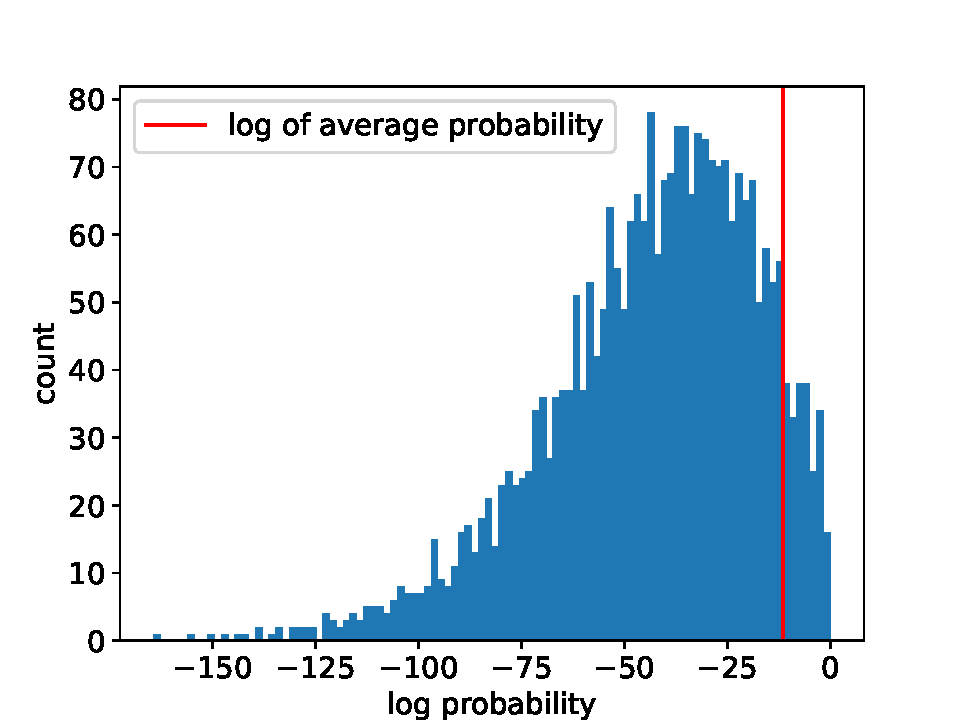
\includegraphics[scale=0.5]{Chapter4/Figs/state_distribution_20_20_all_log_count.pdf}
  \caption{The distribution of the probabilities of all the states for $n=m=20$, using the \DP strategy. Due to the skewness of the distribution, the values are shown on a log-scale.}
  \label{two-thinning-dp-state-distribution}
\end{minipage}\hfill
\begin{minipage}[t]{.48\linewidth}
  \centering
  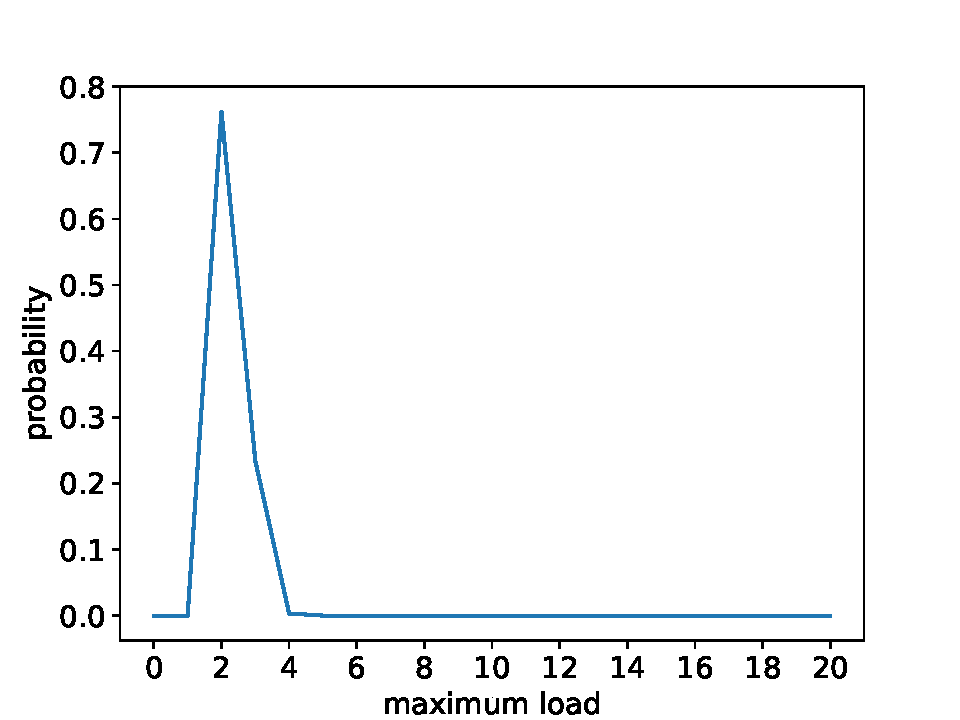
\includegraphics[scale=0.5]{Chapter4/Figs/max_load_distribution_20_20.pdf}
  \caption{The distribution of the final maximum loads for $n=m=20$, using the \DP strategy.}
  \label{two-thinning-dp-maxload-distribution}
\end{minipage}
\end{figure}


\subsection{Deep Q-Learning Analysis}


\subsubsection{Hyperparameter Analysis}


The Weights and Biases tool~\cite{biewald2020wandb} provides hyperparameter importance analysis. It calculates the correlation coefficient between the hyperparameters and the score, for each hyperparameter (green is positive, red is negative). To capture interactions between hyperparameters and also non-linear relationships, it additionally provides an importance score which is calculated based on Random Forests~\cite{biewald2020wandb}. Table~\ref{two-thinning-hyperparameter-importance} -- which is based on the tool -- shows the top $5$ hyperparameters based on the importance score.


We can observe that for \TwoThinning the most important hyperparameter is to use the normalised domain, which was discussed in Section~\ref{normalised-domain}. Also, limiting the maximum threshold that the agent can use efficiently restricts the search space, as discussed in Section~\ref{dqn-implmentation-two-thinning}. As can be seen in Appendix~\ref{hyperparameters}, the ideal maximum threshold is in fact around the target expected maximum load we want to achieve (which can be estimated in general based on theoretical results).



\newcommand{\Progress}[2]{
\begin{tikzpicture}
\draw[fill=#2!10!white] (0,0) rectangle (5, 0.3);
\draw[fill=#2!50!white] (0,0) rectangle (5 * #1, 0.3);
\end{tikzpicture}
}

\begin{table}
\begin{center}
\begin{tabular}{lcc}
 \textbf{Hyperparameter} & \textbf{Importance} & \textbf{Correlation} \\
 \addlinespace[0.2cm]
 \texttt{use\_normalised} & \Progress{0.362}{blue} & \Progress{0.602}{green} \\
 \texttt{max\_threshold} & \Progress{0.141}{blue} & \Progress{0.496}{red} \\
 \texttt{num\_rnn\_layers} & \Progress{0.07}{blue} & \Progress{0.239}{green} \\
 \texttt{rnn\_hidden\_size} & \Progress{0.069}{blue} & \Progress{0.166}{green} \\
 \texttt{pre\_train\_episodes} & \Progress{0.06}{blue} & \Progress{0.103}{red} \\
\end{tabular}
\caption{\TwoThinning hyperparameter importance~\cite{biewald2020wandb} for $n=20$, $m=400$.}
\label{two-thinning-hyperparameter-importance}
\end{center}
\end{table}




\subsubsection{Training}


\begin{figure}[h]
    \centering
    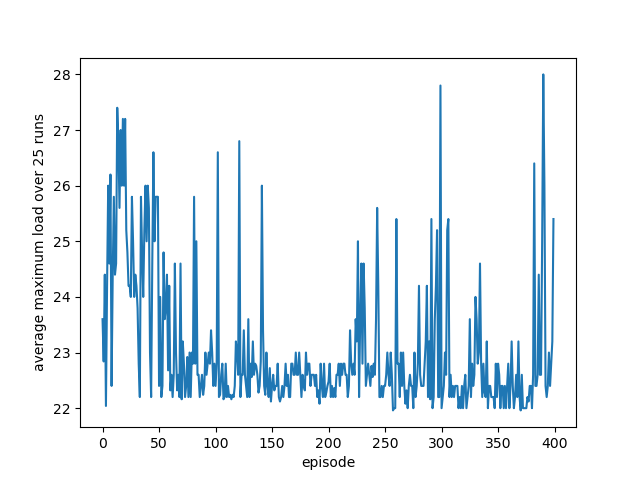
\includegraphics[scale=0.6]{Chapter4/Figs/training_progression_20_400.png}
    \caption{\TwoThinning training curve for $n=20$, $m=400$}
     \label{two-thinning-training-curve}
\end{figure}
\NOTE{T}{Maybe if you do some averaging to the plot, one could see a bit more the learning progress. For example, you could take the average maximum load over the first $x$ episodes.}\NOTE{A}{Change png to pdf!}

As shown in Figure~\ref{two-thinning-training-curve}, improvement during training decays very quickly, and the agent is close to its best already at the start. This is again due to the normalised load domain outlined above -- I checked the training curve without the normalised load domain trick as well, and that shows a much more usual training progression, though leading to a worse optimum. The oscillations in the training curve are mostly due to the inherent randomness in evaluation.


Motivated by the fact that in the normalised domain, a constant $0$ threshold is the \MeanThinning strategy, in Figure~\ref{two-thinning-constant-offset} I tried to see if this simple \MeanThinning strategy could be improved by choosing another constant ``offset'', not $0$. For $n=50$, $m=2500$, the best offset is $1$, and it achieves on average a final maximum load of $52.5$, which is very close to the the theoretical minimum $\frac{m}{n}=50$, and also beats the \DQN strategy. It holds for general $n$ and $m$ that the best offset is usually slightly above $0$.

\begin{figure}[h]
    \centering
    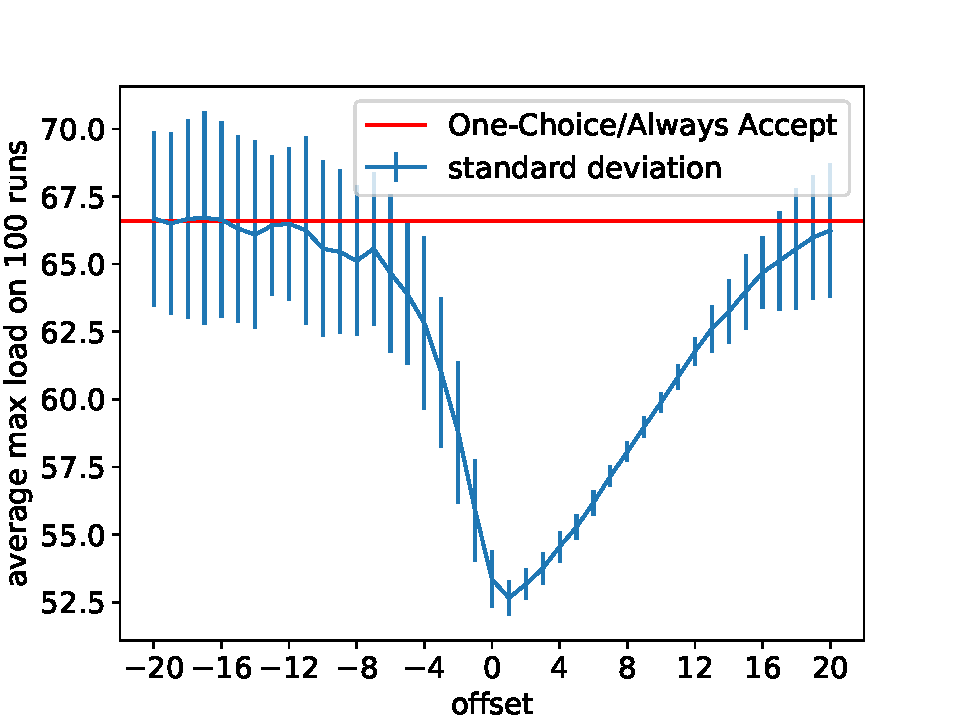
\includegraphics[scale=0.6]{Chapter4/Figs/offset_analysis_50_2500.pdf}
    \caption{Comparing \ConstantOffset strategies for $n=50$, $m=2500$.}
    \label{two-thinning-constant-offset}
\end{figure}


\NOTE{T}{Another interesting ``philosophical'' insight from the figure seems to be that having a too small offset is more detrimental than having a too large offset.}

\NOTE{D}{!!Can you also try $n = 10^4$ and $m = 10^6$ (or larger)?}


The Deep-Q Learning algorithm -- which is as shown above, statistically significantly better than Mean-Thinning -- in fact often learns a strategy similar to a \ConstantOffset strategy, as can be seen in Figure \ref{two-thinning-dqn-thresholds}. The short sporadic ``jumps'' are very challenging for the agent to get rid of, due to the reasons outlined in Section~\ref{two-thinning-comparison}. To avoid this, future work could constrain the agent to change (and only increase) the threshold by at most $1$ after each ball, which is motivated by Conjecture~\ref{conjecture: two-thinning-smooth-threshold}.


\begin{conjecture}\label{conjecture: two-thinning-smooth-threshold}
There exists an optimal (slicing) strategy such that its chosen thresholds are changed by at most $1$ in any step during an execution.
\end{conjecture}


\begin{remark}
Together with Conjecture~\ref{conjecture: two-thinning-increasing-threshold} these would imply an optimal strategy whose threshold either stays the same or increases by $1$ in each step.
\end{remark}


\begin{figure}[h]
    \centering
    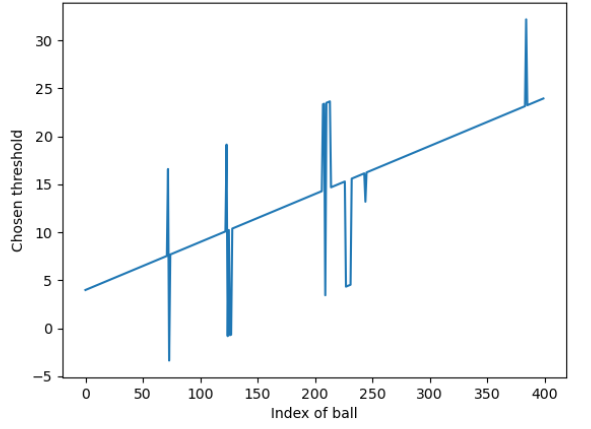
\includegraphics[scale=0.6]{Chapter4/Figs/dqn_learnt_thresholds.png}
    \caption{Analysis of the chosen thresholds of the \DQN strategy for a run of $n=20$, $m=400$.}
    \label{two-thinning-dqn-thresholds}
\end{figure}



\section{\KThinning}



\subsection{Comparison of Strategies}


Since the drawback (TLE) of the \DP strategy has already been highlighted for \TwoThinning, I decided to focus on smaller cases here where a full comparison is feasible and highlight other patterns related to the choice of $k$.


\begin{table}[h!]
\centering
\resizebox{\textwidth}{!}{%
\begin{tabular}{|l|c|c|c|c|c|c|c|c|}
\hline
                                & \multicolumn{4}{c|}{$n=5$} & \multicolumn{4}{c|}{$n=25$}\\ \hline
                                & \multicolumn{4}{c|}{$m=20$} & \multicolumn{4}{c|}{$m=50$}\\ \hline
Strategy                                & $k=2$ & $k=3$ & $k=5$ & $k=10$ & $k=2$ & $k=3$ & $k=5$ & $k=10$ \\ \hline
\AlwaysAccept & 7.73 $\pm$ 0.11 & 7.76 $\pm$ 0.11 & 7.59 $\pm$ 0.11 & 7.67 $\pm$ 0.11 & 5.82 $\pm$ 0.09 & 5.79 $\pm$ 0.08 & 5.83 $\pm$ 0.09 & 5.86 $\pm$ 0.09 \\ \hline \LocalRewardOptimiser & \textbf{6.09 $\pm$ 0.05} & 5.74 $\pm$ 0.04 & 5.41 $\pm$ 0.04 & 5.13 $\pm$ 0.03 & 4.17 $\pm$ 0.04 & 3.73 $\pm$ 0.04 & 3.20 $\pm$ 0.04 & 3.00 $\pm$ 0.01 \\ \hline \Quantile & 6.23 $\pm$ 0.05 & 5.99 $\pm$ 0.04 & 5.58 $\pm$ 0.04 & 5.17 $\pm$ 0.03 & 4.36 $\pm$ 0.06 & 3.66 $\pm$ 0.05 & 3.12 $\pm$ 0.03 & \textbf{3.00 $\pm$ 0.00} \\ \hline \DP & 6.13 $\pm$ 0.05 & \textbf{5.73 $\pm$ 0.04} & \textbf{5.39 $\pm$ 0.04} & \textbf{5.11 $\pm$ 0.03} & \textbf{4.08 $\pm$ 0.04} & \textbf{3.63 $\pm$ 0.04} & \textbf{3.10 $\pm$ 0.03} & \textbf{3.00 $\pm$ 0.00} \\ \hline \Threshold & 6.56 $\pm$ 0.06 & 6.29 $\pm$ 0.05 & 6.14 $\pm$ 0.04 & 5.92 $\pm$ 0.03 & 4.53 $\pm$ 0.05 & 4.19 $\pm$ 0.04 & 3.92 $\pm$ 0.03 & 3.96 $\pm$ 0.03 \\ \hline \DQN & 6.67 $\pm$ 0.07 & 5.87 $\pm$ 0.05 & 5.60 $\pm$ 0.05 & 5.22 $\pm$ 0.04 & 4.51 $\pm$ 0.05 & 3.95 $\pm$ 0.05 & 3.42 $\pm$ 0.04 & 3.04 $\pm$ 0.02 \\ \hline 
\end{tabular}}

\caption{Average maximum load of \KThinning strategies with $95\%$ confidence intervals}
\label{tab:k-thinning-comparison}
\end{table}


Intuitively, the larger $k$ is, the better a strategy can do, and the table confirms it for most of the strategies. We can see from the table that the \Quantile and \LocalRewardOptimiser strategies are almost as good as the \DP strategy for most values of $n$, $m$ and $k$, even though neither of those strategies consider future rewards. For large $k$ ($5$ or $10$) and not too large $n$, strategies can control with high probability where to place the ball. Nevertheless, this kind of advantage is much easier to exploit by a manual algorithm, than to learn by Deep Q-Learning.



\subsection{Theoretical Analysis}


In Figure~\ref{k-thinning-dp-maxload} we can see how the value of $k$ influences the (optimal) DP Strategy. While there is a large improvement from $k=2$ to $k=3$ (e.g. the probability of $\mathrm{maxload}=6$ becomes negligible), we can observe diminishing returns by further increasing $k$.


\begin{figure}[h]
    \centering
    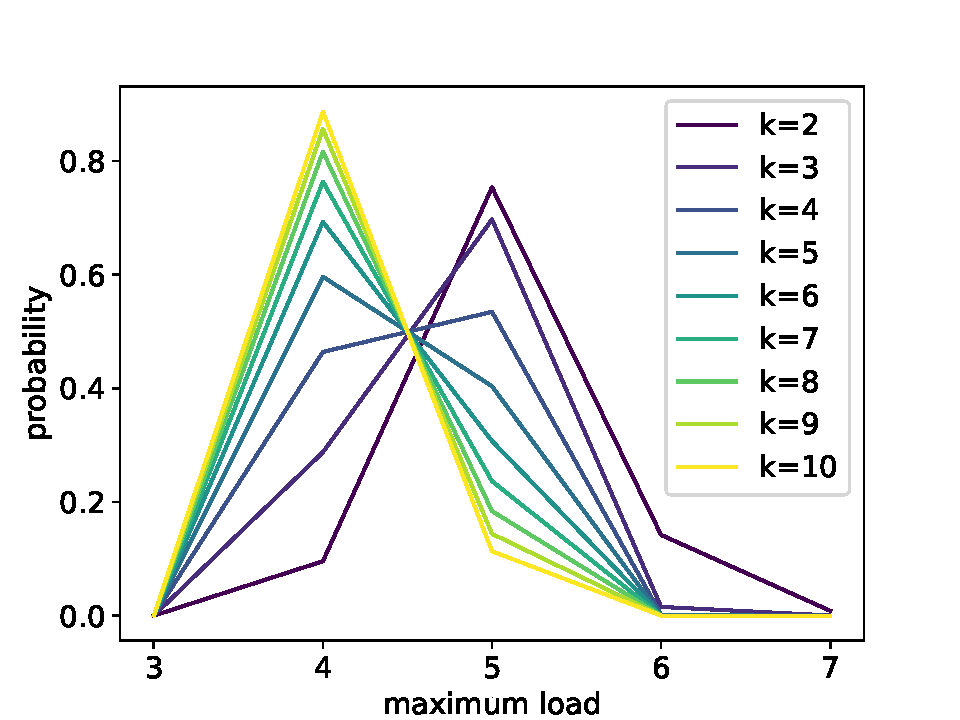
\includegraphics[scale=0.6]{Chapter4/Figs/k_thinning_max_load_distribution_5_20.pdf}
    \caption{Analysis of the final maximum load distribution of the DP strategy for $n=20$, $m=400$ and different values of $k$.}
    \label{k-thinning-dp-maxload}
\end{figure}
\NOTE{T}{Better to use some color scheme (red to green) when transitioning from $k=2$ to $k=10$}

Now I present a lemma about optimal strategies:

\begin{lemma} \label{lemma: k-thinning-monotone}
There exists an optimal monotone strategy.
\end{lemma}

The proof is similar in structure to the proof of Lemma~\ref{lemma: thresholdproperty} for \TwoThinning. We first need a notion of inversions for \KThinning slicing strategies as well:


\begin{definition} [\KThinning inversions]
For a strategy $f$, we call a (sorted) load vector $v$ and two integers $0\leq i<j<k-2$ an inversion if $h^f(v,i)>h^f(v,j)$. Let's denote the number of inversions of $f$ by $J^f$, and the number of inversions for a fixed $v$ by $J^f_v$.
\end{definition}


\begin{proof}[Proof of Lemma~\ref{lemma: k-thinning-monotone}]
    The proof proceeds by contradiction. Assume that there is no monotone optimal strategy. Take an optimal non-monotone strategy $f$, with the least number of inversions $J^f$. Since $f$ is not monotone, $J^f>0$, so we can take a(n arbitrary) $v$ with $J^f_v>0$. Let $c=\argmax_j h^f(v,j)>h^f(v,j+1)$. Let's define a strategy $g$ such that $h^g(v,c)=h^f(c+1)$, $h^g(v,c+1)=h^f(v,c)$ (``swap'' action) and otherwise acting like $f$. Now I show that for any load vector $w$, $P^f_w \preccurlyeq P^g_w$.
    
    When $w\neq v$, $P^f_w=P^g_w$ by construction, so $P^f_w \preccurlyeq P^g_w$. For $w=v$, let's denote the ratio of bins with load $>x$ as $r(x)$. Then, applying the rules of \KThinning, $$P^f_v[i]=\sum_{j=0}^{k-1} \left(\prod_{l=0}^{j-1} r(h^f(v,l))\right)\cdot\frac{1}{n}\cdot\mathbbm{1}_{v[i]\leq h^f(v,j)}$$ because the ball can be allocated to bin $i$ after $j$ rejected balls if the next bin chosen is $i$ and its load is less than or equal to the next threshold. By case splitting on the load of bin $i$, we get
    
    $$P^g_v[i]= \begin{cases}
        P^f_v[i]+\left(\prod_{l=0}^{c-1} r(h^f(v,l))\right)\cdot(r(h^f(v,c+1))-r(h^f(v,c))), & \text{for } v[i]\leq h^f(v,c+1),\\
        P^f_v[i]+\left(\prod_{l=0}^{c-1} r(h^f(v,l))\right)\cdot(r(h^f(v,c+1))-1), & \text{for } h^f(v,c+1)<v[i]\leq h^f(v,c),\\
        P^f_v[i], & \text{for } h^f(v,c)<v[i].
    \end{cases}$$
    
    after some algebraic simplification, showing that only a few terms of the sum in $P_v^f$ are affected by the ``swap''\NOTE{A}{This is a bit tedious to explain how I got this sum but there is really nothing fancy going on, just applying the rules of \KThinning and doing some simplification. Should I explain anymore? Or is it convincing enough?}. Note that $r(h^f(v,c+1))-r(h^f(v,c))>0$ because $h^f(v,c+1)<h^f(v,c)$ by definition of $c$, and similarly $r(h^f(v,c+1))-1<0$ because $r$ is a ratio. Hence, probability has only been moved to the left after the ``swap'', so $P^f_v \preccurlyeq P^g_v$\NOTE{A}{I could write this sentence one down formally, is it worth the space or this handwavy sentence is enough?}.
    
    Since $P^f_w\preccurlyeq P^g_w$ for any load vector $w$, Lemma~\ref{lemma: majorisation-implies-better} implies $E^g\leq E^f$. $J^g=J^f-1<J^f$, because the ``swap'' removed the inversion between $c$ and $c+1$ and didn't introduce any new inversions apart from changing the role of $c$ and $c+1$ (see Figure~\ref{k-thinning-swap-action}). Hence, either $E^g<E^f$, or $E^g=E^f$ but $J^g<J^f$, contradicting the original assumption.
\end{proof}


\begin{figure}
    \centering
    %\includegraphics{}
    \caption{The ``swap'' action for \KThinning}
    \label{k-thinning-swap-action}
\end{figure}

\begin{remark}
Lemma~\ref{lemma: k-thinning-monotone} has been verified by showing that this property holds for the (optimal) \DP strategy for several combinations of $n$, $m$ and $k$.
\end{remark}


\subsection{Deep Q-Learning Analysis}



\subsubsection{Hyperparameter Analysis}



\begin{table}
\begin{center}
\begin{tabular}{lcc}
 \textbf{Hyperparameter} & \textbf{Importance} & \textbf{Correlation} \\
 \addlinespace[0.2cm]
 \texttt{optimise\_freq} & \Progress{0.138}{blue} & \Progress{0.42}{red} \\
 \texttt{target\_update\_freq} & \Progress{0.133}{blue} & \Progress{0.124}{green} \\
 \texttt{eps\_decay} & \Progress{0.088}{blue} & \Progress{0.051}{red} \\
 \texttt{pre\_train\_episodes} & \Progress{0.084}{blue} & \Progress{0.293}{green} \\
 \texttt{batch\_size} & \Progress{0.074}{blue} & \Progress{0.205}{red} \\
\end{tabular}
\caption{\KThinning hyperparameter importance~\cite{biewald2020wandb} for $n=20$, $m=400$.}
\label{k-thinning-hyperparameter-analysis}
\end{center}
\end{table}


We can observe in Table~\ref{k-thinning-hyperparameter-analysis} that the normalised load domain trick is not as crucial for \KThinning as it was for \TwoThinning\NOTE{A}{Mention some bullshit possible reason?}. On the other hand, the analysis suggests more frequent optimisation update steps and more curriculum learning (pretraining) episodes. 


\subsubsection{Training}


\begin{figure}[h]
    \centering
    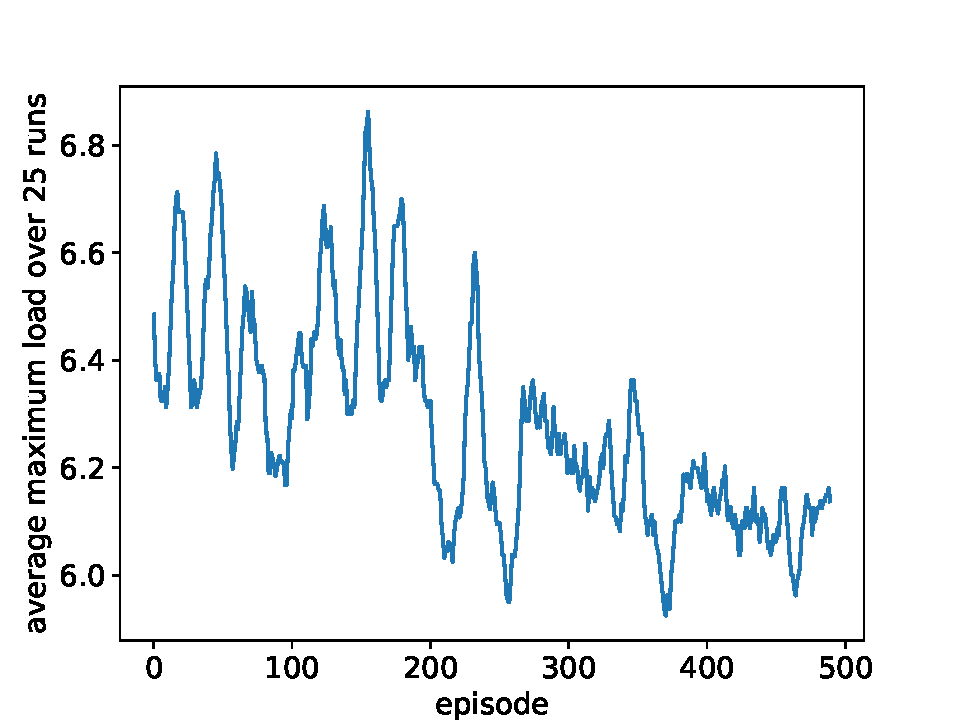
\includegraphics[scale=0.6]{Chapter4/Figs/training_progression_rolling_window_5_25_3.pdf}
    \caption{\KThinning training curve for $n=5$, $m=25$, $k=3$, with $10$ episodes wide rolling window averaging for readability purposes.}
    \label{k-thinning-training-curve}
\end{figure}


The training progression shown in Figure~\ref{k-thinning-training-curve} is similar to \TwoThinning, so I do not discuss it any further.


\section{\GraphicalTwoChoice}


\subsection{Comparison of Strategies}
\begin{table}[h!]
\centering
\resizebox{\textwidth}{!}{%
\begin{tabular}{|l|c|c|c|c|c|c|c|c|c|}
\hline
                                & \multicolumn{3}{c|}{$n=4$} & \multicolumn{3}{c|}{$n=16$} & \multicolumn{3}{c|}{$n=32$}\\ \hline
                                & \multicolumn{3}{c|}{$m=25$} & \multicolumn{3}{c|}{$m=50$} & \multicolumn{3}{c|}{$m=32$}\\ \hline
Strategy                                & Cycle & Hypercube & Complete & Cycle & Hypercube & Complete & Cycle & Hypercube & Complete \\ \hline
\Greedy & 7.06 $\pm$ 0.02 & 7.06 $\pm$ 0.02 & 7.19 $\pm$ 0.04 & \textbf{4.75 $\pm$ 0.05} & \textbf{4.51 $\pm$ 0.05} & \textbf{4.40 $\pm$ 0.05} & \textbf{2.40 $\pm$ 0.05} & \textbf{2.33 $\pm$ 0.04} & \textbf{2.26 $\pm$ 0.04} \\ \hline \Random & 8.96 $\pm$ 0.12 & 8.97 $\pm$ 0.12 & 8.84 $\pm$ 0.11 & 6.49 $\pm$ 0.09 & 6.62 $\pm$ 0.10 & 6.69 $\pm$ 0.10 & 3.49 $\pm$ 0.06 & 3.52 $\pm$ 0.07 & 3.50 $\pm$ 0.06 \\ \hline \LocalRewardOptimiser & 7.12 $\pm$ 0.03 & 7.11 $\pm$ 0.03 & 7.25 $\pm$ 0.04 & 4.87 $\pm$ 0.06 & 4.77 $\pm$ 0.05 & 4.74 $\pm$ 0.05 & 2.53 $\pm$ 0.05 & 2.44 $\pm$ 0.04 & 2.38 $\pm$ 0.04 \\ \hline \DP & \textbf{7.04 $\pm$ 0.02} & \textbf{7.03 $\pm$ 0.01} & \textbf{7.17 $\pm$ 0.03} & TLE & TLE & TLE & TLE & TLE & TLE \\ \hline \DQN & 7.11 $\pm$ 0.03 & 7.11 $\pm$ 0.03 & 7.31 $\pm$ 0.05 & 4.88 $\pm$ 0.07 & 4.53 $\pm$ 0.05 & 4.50 $\pm$ 0.05 & 2.68 $\pm$ 0.06 & 2.54 $\pm$ 0.05 & 2.60 $\pm$ 0.06 \\ \hline 
\end{tabular}}

\caption{Average maximum load of \GraphicalTwoChoice strategies with $95\%$ confidence intervals\protect\footnotemark}
\label{tab:graphical-two-choice-comparison}
\end{table}

\footnotetext{Note that for $n=4$, the \CycleGraph and the \HypercubeGraph are the same.}

The most important conclusions from Table~\ref{tab:graphical-two-choice-comparison} are:

\begin{itemize}
    \item The \Greedy strategy is not exactly optimal, as can be seen from the $n=4$ case (I will provide an explicit counterexample in Lemma~\ref{lemma: greedy-suboptimal}). On the other hand, it is close to the performance of the \DP strategy, and when that is not applicable, \Greedy is by far the best.
    \item While for larger $n$, agreeing with the intuition the \CompleteGraph is the most favourable for \Greedy, it works better on the \CycleGraph for $n=4$. 
    \item The \DQN strategy performs performs consistently, but it cannot always exploit the subtle suboptimalities of \Greedy. Its performance is comparable to the performance of the \LocalRewardOptimiser strategy.
    
\end{itemize}


\subsection{Theoretical Analysis}

First I prove the most surprising result of this section.

\begin{lemma} \label{lemma: greedy-suboptimal}
There exists a graph, such that the \Greedy strategy is suboptimal with respect to the expected final maximum load of \GraphicalTwoChoice.
\end{lemma}

\begin{proof}
Using the \DP strategy for the \CycleGraph with $n=4$ bins $m=6$ balls, I found a state $s$ (i.e.\ a load vector $v$ and edge $e$), where choosing the less loaded bin is suboptimal. Denoting the nodes as ($1$-based) indices in the load vector, the counterexample state is $v=(0,1,0,2)$,  $e=(2,3)$ i.e.\ there is an edge between the second and third bin. \Greedy would choose the third bin, but if all the later edges are $(3,4)$, $\mathrm{maxload}>2$ cannot be avoided (see Figure~\ref{greedy-counterexample}). On the other hand, by choosing the second bin and then picking the odd-indexed endpoints of the later edges, the maximum load will always be $2$. Therefore, the expected final maximum load of choosing the second bin (and then playing optimally) is $2.0$, while that of choosing the third bin is between $2.0$ and $3.0$.
\end{proof}



\begin{figure}
    \centering
    \begin{tikzpicture}
    \Tree [.$(0,\underline{\mathbf{1}},\underline{\mathbf{0}},2)$
    [.$(0,1,\underline{\mathbf{1}},\underline{\mathbf{2}})$
    [.$(0,1,\underline{\mathbf{2}},\underline{\mathbf{2}})$
    [.$(0,1,3,2)$ ] $\ldots$ ] $\ldots$ ]
    [.$(0,2,0,2)$ $\ldots$ ]]
    \end{tikzpicture}
    \caption{Counterexample for the optimality of \Greedy, showing that choosing the second bin can lead to a maximum load of $3$ while choosing the third bin cannot.}
    \label{greedy-counterexample}
\end{figure}



To better understand the impact of the graph structure on \Greedy, I analysed the relationship between the degree $d$ of the graph and how well \Greedy performs on it. I created $1000$ random regular graphs for each degree $1\leq d \leq 31$ of the $n=m=32$ case. \NOTE{T}{Very interesting... I would have hoped that maybe for $d \approx 15$ or so you would get the best performance, which in a way, would generalise the cycle for small values of $n$. Andor: Interesting idea, I don't know how to generalise the cycle for smalle values of $n$.} We can see in Figure~\ref{greedy-random-regular-analysis} that smaller degrees hurt \Greedy, but after around $d=20$, the performance no longer improves.


\begin{figure}[h]
    \centering
    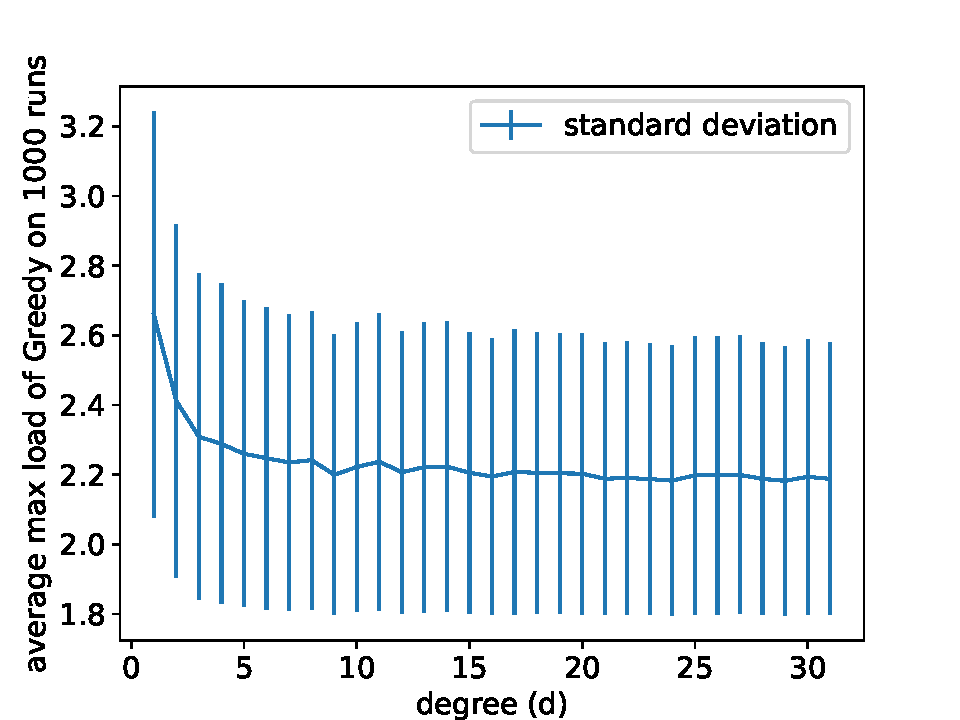
\includegraphics[scale=0.6]{Chapter4/Figs/greedy_degree_analysis_32_32.pdf}
    \caption{Relating the degree of the graph to the performance of Greedy for $n=m=32$.}
    \label{greedy-random-regular-analysis}
\end{figure}


\subsection{Deep Q-Learning Analysis}

To better understand the difficulty in finding an optimal strategy, I extended the \CycleGraph counterexample from Lemma ~\ref{lemma: greedy-suboptimal} to load vectors of the form $(0, a, 0, b)$, with the next edge still going between the second and third bins. Figure~\ref{greedy-counterexample-analysed} and Figure~\ref{greedy-counterexample-analysed-for-dqn} show that the shape of the region containing counterexamples to the \Greedy strategy is difficult to characterise, and to precisely learn by RL. By using the $\Phi_{neigh}$ potential function for Deep Q-Learning, the agent is guided towards choosing second bin, and by using a graph-oblivious potential (e.g.\ $\Phi_{max}$), the agent is guided towards choosing the third bin. Therefore, neither of the potential functions is perfect. We can indeed see in Figure~\ref{greedy-counterexample-analysed-for-dqn} that the DQN could not learn the exact pattern, though there is some resemblance.


\begin{figure}
\centering
\begin{minipage}[t]{.48\linewidth}
  \centering
  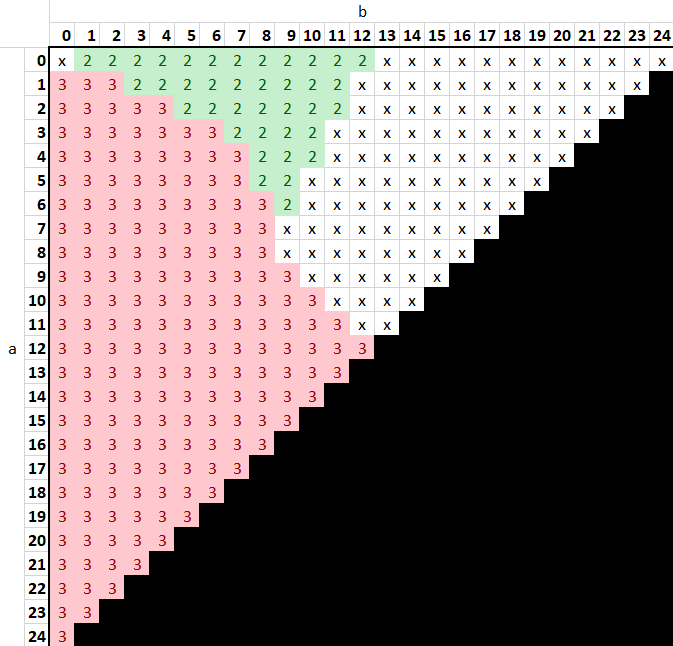
\includegraphics[scale=0.45]{Chapter4/Figs/0a0b_4_25_analysis.png}
  \caption{The optimal decisions for the \CycleGraph with $n=4$, $m=25$, load vector $(0,a,0,b)$ and edge $(2,3)$. Green indicates choosing the second bin is better, red indicates choosing the third bin is better, and $x$ indicates that they have the same expected score.}
  \label{greedy-counterexample-analysed}
\end{minipage}\hfill
\begin{minipage}[t]{.48\linewidth}
  \centering
  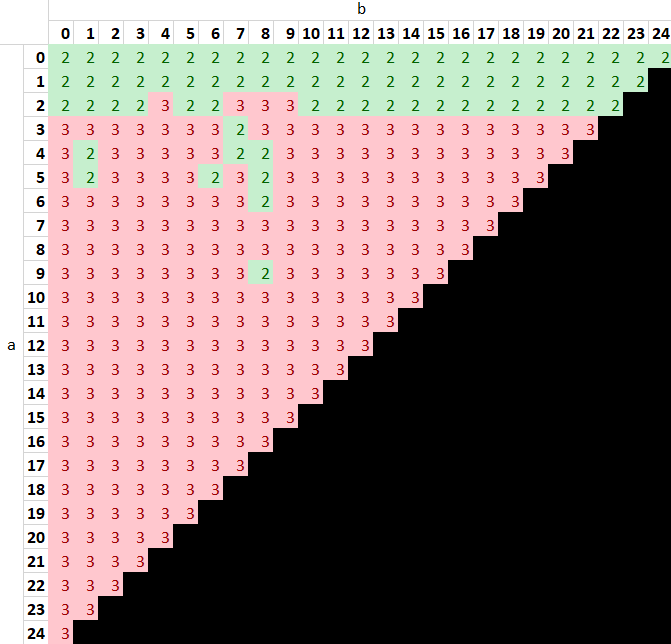
\includegraphics[scale=0.45]{Chapter4/Figs/0a0b_4_25_analysis_dqn.png}
  \caption{The decisions made by the \DQN strategy in the situation from Figure~\ref{greedy-counterexample-analysed}.}
  \label{greedy-counterexample-analysed-for-dqn}
\end{minipage}
\end{figure}



\subsubsection{Hyperparameter Analysis}


Analysing Table~\ref{graphical-two-choice-hyperparameter-importance}, the negative correlation of ``hidden\_size'' and ``num\_lin\_layers'' with the score suggests that adding more parameters to the DQN does not help. 


\begin{table}
\begin{center}
\begin{tabular}{lcc}
 \textbf{Hyperparameter} & \textbf{Importance} & \textbf{Correlation} \\
 \addlinespace[0.2cm]
 \texttt{pre\_train\_episodes} & \Progress{0.207}{blue} & \Progress{0.450}{green} \\
 \texttt{num\_lin\_layers} & \Progress{0.190}{blue} & \Progress{0.344}{red} \\
 \texttt{hidden\_size} & \Progress{0.162}{blue} & \Progress{0.462}{red} \\
 \texttt{optimise\_freq} & \Progress{0.074}{blue} & \Progress{0.333}{red} \\
 \texttt{target\_update\_freq} & \Progress{0.071}{blue} & \Progress{0.124}{red} \\
\end{tabular}
\caption{\GraphicalTwoChoice hyperparameter importance for the \CycleGraph with $n=4$ and $m=25$ \cite{biewald2020wandb}}
\label{graphical-two-choice-hyperparameter-importance}
\end{center}
\end{table}


\subsubsection{Training}

Figure~\ref{graphical-two-choice-training-curve} shows a much steadier improvement during training for \GraphicalTwoChoice than what we saw for \TwoThinning and \KThinning. This is mostly because there is no reasonable easy-to-learn initial strategy for \GraphicalTwoChoice with the chosen MDP formulation, unlike the \ConstantOffset strategies for \TwoThinning.

\begin{figure}[h] 
    \centering
    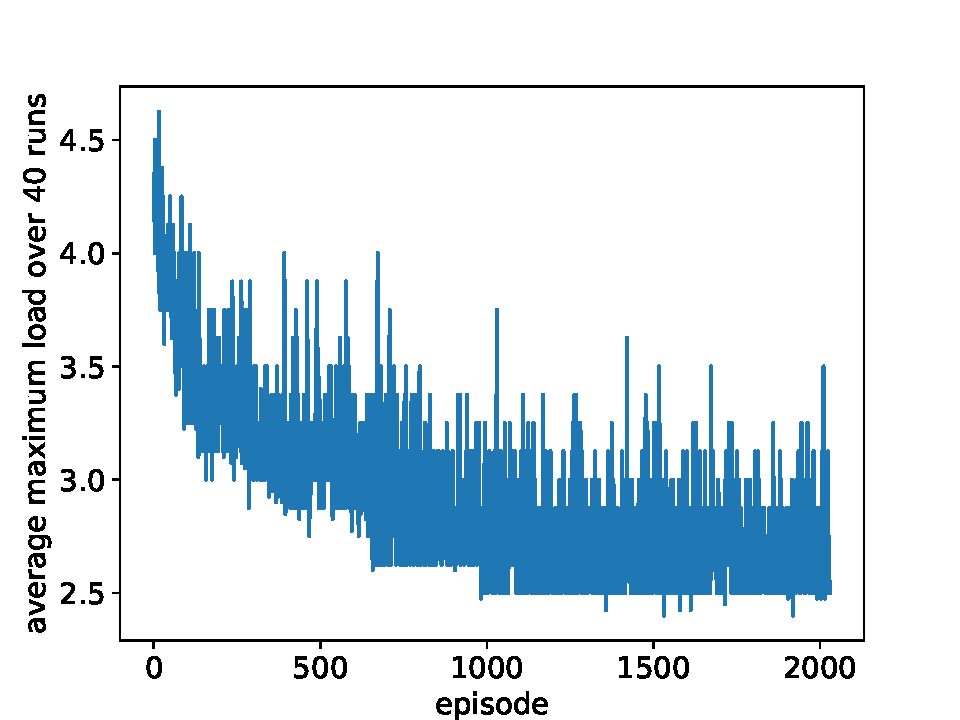
\includegraphics[scale=0.6]{Chapter4/Figs/training_progression_hypercube_32_32.pdf}
    \caption{\GraphicalTwoChoice training curve for the \CycleGraph with $n=m=32$.}
    \label{graphical-two-choice-training-curve}
\end{figure}

